% ---------------------------------------------------------------------
% CILAMCE 2018, 11-14 November 2018, Paris/Compiègne, France
% ---------------------------------------------------------------------
\documentclass{cilamce}

% ---------------------------------------------------------------------
\title{Efficient LBM on GPUs for dense moving objects using immersed boundary condition}
% ---------------------------------------------------------------------
\author{Jo\"el Beny$^1$, Jonas L\"att$^2$}
% ---------------------------------------------------------------------
\address{%
$^1$ Universit\'e de Gen\`ve, Geneva, Switzerland, Joel.Beny@etu.unige.ch\\
$^2$ Universit\'e de Gen\`ve, Geneva, Switzerland, Jonas.Latt@unige.ch
}
% ---------------------------------------------------------------------
\begin{document}
% ---------------------------------------------------------------------
\maketitle
% ---------------------------------------------------------------------

There exists an increasing interest for using immersed boundary methods (IBMs)~\cite{peskin} to model moving objects in computational fluid dynamics, because this approach does not require any adaptation of the fluid mesh, and is therefore particularly efficient. This approach is particularly frequently proposed in combination with the lattice Boltzmann methods (LBM)~\cite{bgk, lbm}; it fits in an elegant way into the framework of this method, and yields impressive parallel performance.

It has also become quite common to accelerate LBM simulations with the use of Graphics Processing Units (GPUs)~\cite{tolke}, as the algorithm of the method adjusts naturally to the architecture of this platforms, and it is not uncommon that speedups of 1-2 orders of magnitude at equal financial cost or energy consumption are observed, as compared to classical CPUs. IBM algorithms are however more difficult to translate to GPUs, because their complex memory access pattern conflicts with a GPUs strategy of broadcasting data to a large number of GPU cores in single memory accesses. In the existing literature, GPU implementations of LBM-IBM codes are therefore restricted to situations in which the immersed surfaces are very small compared to the total number of fluid cells~\cite{lara}, as is often the case in exterior flow simulations around an obstacle. This assumption is however not valid in many other cases of interest, as for example the simulation of deformable red blood cells, for which many authors have adopted the LBM and IBM as their method of choice. Indeed, red blood cells fill the blood volume densely, and the immersed surfaces contribute substantially to the overall computational cost.

We propose new methods for the implementation of a LBM-IBM on GPUs in the CUDA language~\cite{cuda}, which allow to handle a substantially larger immersed surface with acceptable performance than previous implementations. For test purposes, we consider the case of a single or multiple rotating propellers in a fluid. The methods is applied to a direct-forcing flavor of the IBM as proposed by Ota, Suzuki, and Inamuro~\cite{ota}. In this method, the surface is represented by a certain number of points with Lagrangian coordinates, which interact with the fluid within a given kernel through a force term. The algorithm is iterative, to achieve agreement between the effect of neighboring, overlaping kernels, and each iteration is split into two parts: (1) a fluid $\rightarrow$ surface data transmission, during which the flow velocity is interpolated onto the immersed surface, and (2) a surface $\rightarrow$ fluid data transmission, during which the surface acts onto the fluid through a force term to enforce the boundary condition.

Our efficient GPU algorithm is based on three key ingredients:
\begin{enumerate}
    \item Single-population LBM implementation: the populations are allocated only once in GPU memory (while a straightforward GPU implementation would allocate ``incoming'' and ``outgoing'' populations in separate arrays). The so-called ``AA-pattern''~\cite{aa} is used, which is thread safe and therefore compatible with the multi-core framework of a GPU.
    \item The two steps of an IBM iteration (fluid $\rightarrow$ surface vs. surface $\rightarrow$ fluid) are parallelized separately, and thus dispatched to different GPU cores, to achieve a best memory access pattern for each of them.
    \item The IBM algorithm is not applied to the full fluid domain, but to a restricted domain comprising all IBM kernels, to optimize the usage of the available GPU cores. Two strategies are tested, one applying the method to a cube around the immersed object (``the box strategy''), and one restricted to the exact number of fluid nodes that are subject to the IBM force, which need to be recomputed at every time step to adjust to the moving object (``the kernel stragegy'').
\end{enumerate}

The figure below illustrates the geometry of the propeller we use in the test case, as well as the fluid cells which dispatched to the GPU cores for the IBM algorithm, in case the above-mentioned ``kernel strategy'' is used.

\begin{center}
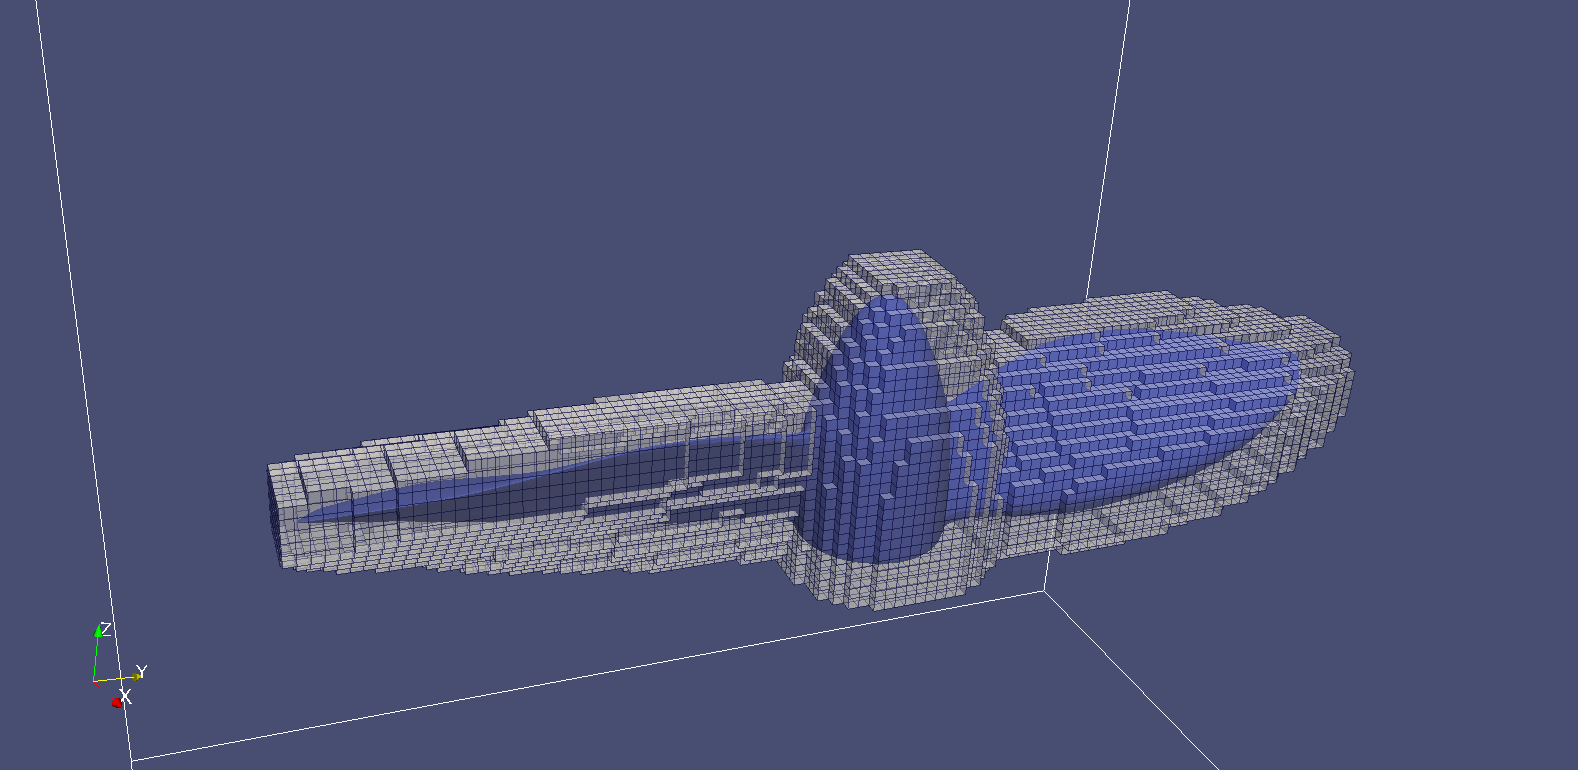
\includegraphics[width=.5\textwidth]{kernel-strategy.png}
\end{center}

Our implementation was executed on a NVIDIA Tesla P100-PCIE GPU with 3584 CUDA cores and a maximum clock rate of 1.33 GHz. The speed was compared to a CPU implementation proposed by the Palabos library~\cite{palabos}, executed on an Intel Xeon E5-2620 12-core CPU at 2 GHz (all 12 cores are being exploited by Palabos with help of MPI parallelism). The performance is assessed by means of Million Lattice-Site-Updates per Second (MLUPS), the number of lattice nodes for which a full collision-streaming cycle is compared, divided by $10^{-6}$. We first simulated a single propeller, represented by 3930 surface points, embedded in a fluid domain of 160$\times$160$\times$320=8.2 Million fluid cells. In this case, the GPU has a 19-fold speedup as compared to the CPU:

\begin{center}
    \begin{tabular}{l|l|l}
        GPU & 893 MLUPS\\
        CPU & 46.8 MLUPS\\
    \end{tabular}
\end{center}

To test the capability of the implementation to cope with large surfaces, we duplicated the propeller, and ran multiple, independently rotating propellers, as illustrated on the image below:

\begin{center}
    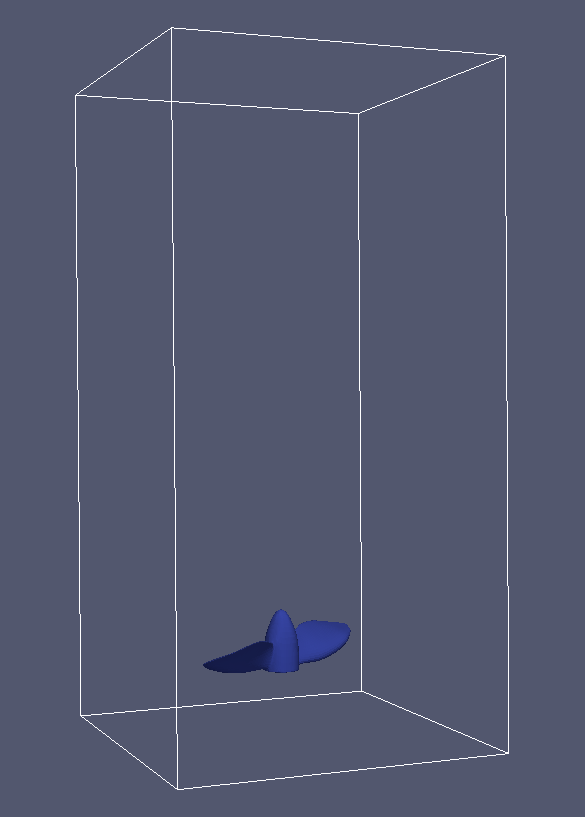
\includegraphics[width=.2\textwidth]{1prop.png}
    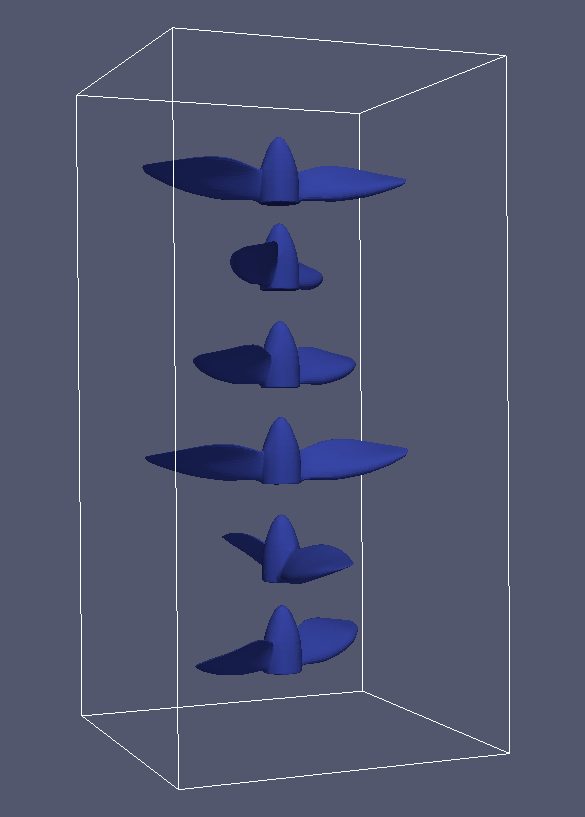
\includegraphics[width=.2\textwidth]{multiprop.png}
\end{center}

The graph illustrates the evolution of the performance as new rotating propellers are added into the fluid. With six propellers, and a total of 23580 immersed surface points, the GPU performance is still outstanding at more than 650 MLUPS.

\begin{center}
    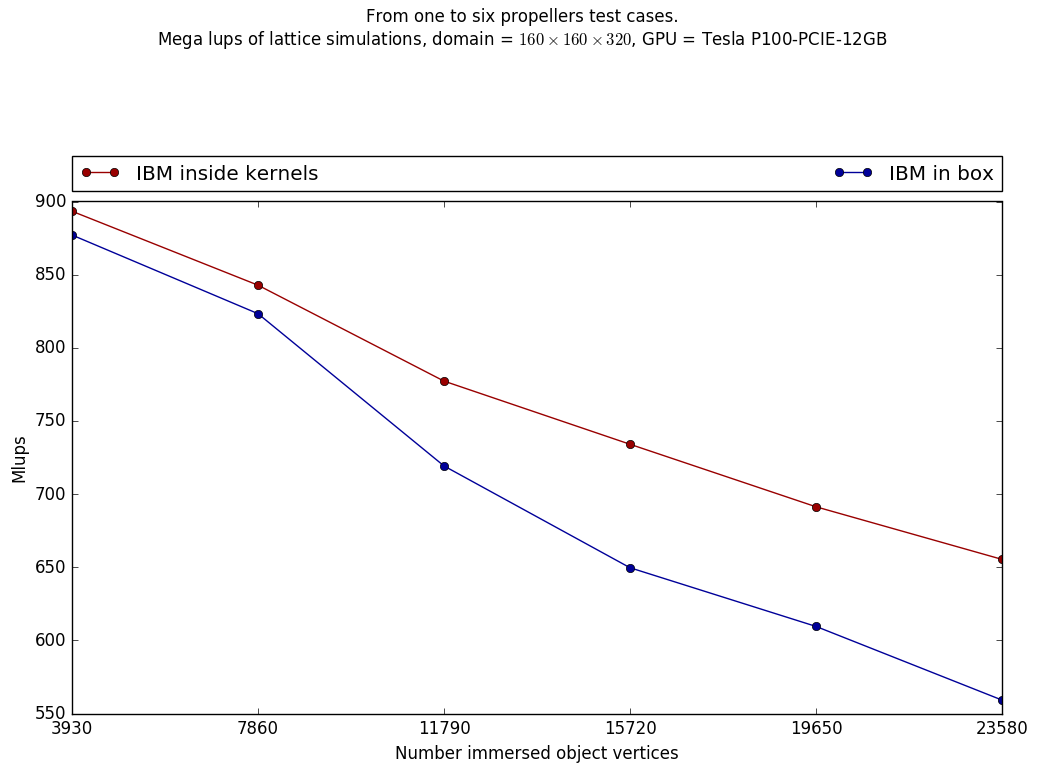
\includegraphics[width=.7\textwidth]{gpu_abst.png}
\end{center}


\begin{thebibliography}{1}
   \bibitem{lbm}
       T. Kr\"uger, H. Kusumaatmaja, A. Kuzmin, O. Shardt, G. Silva, and E.M. Viggen.  The Lattice Boltzmann Method: Principles and Practice.  Graduate Texts in Physics, 2016.

   \bibitem{palabos}
          http://www.palabos.org/

   \bibitem{bgk}
          P. L. Bhatnagar, E. P. Gross, and M. Krook. 
          A Model for Collision Processes in Gases. I. Small Amplitude Processes in Charged and Neutral One-Component Systems. 
          Phys. Rev. 94. 
          51 May 1954

   \bibitem{ota}
          Keigo Ota and Kosuke Suzuki and Takaji Inamuro.
          Lift generation by a two-dimensional symmetric flapping wing: immersed boundary-lattice Boltzmann simulations.
          Fluid Dynamics Research, vol 44, page 045504.
          2012

   \bibitem{peskin}
          Lai M-C and Peskin. 
          An immersed boundary method with formal second-order accuracy and reduced numerical viscosity.
          J. Comput. Phys. 160
          2000

   \bibitem{cuda}
          https://devblogs.nvidia.com/even-easier-introduction-cuda

   \bibitem{cuda2}
          https://www.nvidia.com/content/PDF/fermi\_white\_papers/NVIDIA\_Fermi\_Compute\_Architecture\_Whitepaper.pdf

   \bibitem{lara}
          Pedro Valero-Lara, Alfredo Pinelli, and Manuel Prieto-Matias.
          Accelerating Solid-Fluid Interaction using Lattice-Boltzmann and Immersed Boundary Coupled Simulations on Heterogeneous Platforms.
          Procedia Computer Science, Volume 29, Pages 50--61.
          2014

   \bibitem{tolke}
          Jonas T\"lke.
          Implementation of a Lattice Boltzmann kernel using the Compute Unified Device Architecture developed by nVIDIA. 
          Comput Visual Sci 13:29--39.
          2010

   \bibitem{aa}
          Bailey, P., Myre, J., Walsh, S. D. C., Lilja, D. J., \& Saar, M. O. (2009).
          Accelerating lattice boltzmann fluid flow simulations using graphics processors.
          In ICPP-2009 - The 38th International Conference on Parallel Processing (pp. 550--557). [5362489] DOI: 10.1109/ICPP.2009.38

\end{thebibliography}
% ---------------------------------------------------------------------

% ---------------------------------------------------------------------
\end{document}
% ---------------------------------------------------------------------

